% File SDSS2020_SampleExtendedAbstract.tex
\documentclass[10pt]{article}
\usepackage{sdss2020} % Uses Times Roman font (either newtx or times package)
\usepackage{url}
\usepackage{latexsym}
\usepackage{amsmath, amsthm, amsfonts}
\usepackage{algorithm, algorithmic}
\usepackage{graphicx}
\usepackage{adjustbox}
\graphicspath{{images/}}

\title{Artificial Neural Networks and Deep Learning \\
Homework 1}

\author{
  Nicola Dean \\
  10617541 \\
  {\tt nicola.dean \\
  \tt @mail.polimi.it} \\\And
  Marco Fasanella \\
  10617541 \\
  {\tt marco.fasanella \\
  \tt @mail.polimi.it} \\\And
  Raffaello Fornasiere \\
    10790353 \\
    {\tt raffaello.fornasiere \\
    \tt @mail.polimi.it} \\\And
  Christian Spano \\
  10617541 \\
  {\tt christian.spano \\
  \tt @mail.polimi.it} \\}


\date{}

\begin{document}
\maketitle
%\begin{abstract}

%\end{abstract}

%{\bf Keywords:} VGG16, VGG19, Helpful

\section{Introduction}
In order to touch all the important aspects of the procedure of finding the best solution to this classification problem,
we started from our own self-made model to more sophisticated methodologies.\\
 We can summarize our approaches in:
\begin{itemize}
  \item Vanilla network
  \item Transfer Learning and Fine Tuning
  \item Ensemble method
\end{itemize}
Furthermore in all the attempts made, we used two classes, specifically \textbf{created to automate and support the model creation
procedure}:
\begin{itemize}
  \item Dataset Helper
  \item Model Helper
\end{itemize}
Through the continuous attempts, and support of methods in the two helper classes, we managed to find our best model and
reach 0.8691 accuracy in the competition.


\section{Dataset Helper and Model Helper}
In order to ease the development of our best solution, we thought it would have been useful to create two ad-hoc helper libraries. As a matter of fact, a lot of code is often repeated or many lines of code are needed just to plot or to get insightful results (such as the confusion matrix or the accuracy). In particular, what we did was to create two helpers:
\begin{itemize}
    \item \textbf{Dataset helper}: for dealing with everything related to the dataset; for instance (just for mentioning the most relevant functions) we created functions to perform \textit{augmentation} and \textit{cut-out/cut-mix} of the dataset. Other functions were intended for processing data (e.g., normalization)
    \item \textbf{Model helper}: for dealing with everything related to the models; this helper was intended for easing the construction of models. For instance, we create some functions for plotting insightful graphs (e.g., confusion matrix, residuals, predictions, etc.) and some other functions for managing the models (e.g., save the model in a specified directory or create checkpoints during training)
\end{itemize}
At the end, these helpers indeed turned out to be really helpful. Just with a line we had everything we needed. 

\section{First try: vanilla network}
--NICOLA--
-IMG della rete (dal lab) (magari orizzontale)
risultati
considerazioni
\subsection{Batch Normalization}
A first attempt was also adding a Batch Normalization + Relu Activation Layer before our Pooling layers.\
This lead to poor result due to the fact that the network was too small.

\subsection{Our homemade CNN}
After some attempts on small vanilla networks with poor results we've tried to improve the network by adding some more layers with more filters.
We combined different parameters: kernel size, number of filters, number of layers, units of the dense layers.
After some trials we noticed that we weren't reaching any significant improvement (very low test scores, around 0.5/06 of accuracy).
All of these trials were made with a small dataset (4000 images), but after the work done on augmentation (\ref{subsec:augmentation}) the same model performed much better reaching 0.80/0.85 on test set.
We noticed though the model wasn't much reliable since on codalab it performed around 0,78.


\subsection{Augmentation}\label{subsec:augmentation}
Since vanilla networks weren't providing good results we decided to focus on data.
First of all we decided to generate a number of images so that the ratio $images_{specie_i}/tot_{images}$ was almost the same for each specie $i$.
then we started exploiting all the functionalities of ImageDataGenerator in order to generate as much images as possible so that the network could extract them without overfitting.
By doing this we started reaching higher accuracies deduced that the image dataset shouldn't be smaller then 10k images.
With further search we noticed smaller - but significant - improvements until 25k images.
After that we decided to improve the generalization ability of the network by augmenting the images with CutMix, MixUp, GridMask and Grayscale.
This turned out to be another small but significant improvement on the accuracy, reaching 3/4 percentage points on test accuracy, depending also on the model used.



\subsection{Considerations}
Best result consideration and observations \\
Commento da Christian: qui specifichiamo l'importanza della augmentation e che abbiamo pensato potesse risolvere il problema della bassa accuracy (infatti alla fine è megliorato) + che poi abbiamo espanso con cut-out e cut-mix -- magari dire brevemente il perché, secondo noi, con augmentation/cutout è migliorato.
\section{Transfer Learning and Fine Tuning}
We then noticed that we needed a big change on the approach to use, because the homemade
CNN was performant, but not enough. So \textbf{we started using transfer learning and Fine tuning}

\subsection{Approach: Freezing Layers}
The \textit{modus operandi} that will be used from now is: freezing all layers while training on our augmented dataset the keras.application
CNN, and then unlock a small amount of layers to the second phase of training (fine tuning) as near as possible to the output.
\subsection{VGG16}
The first network we decided to utilize with this approach was VGG16. We started from this network mainly because, generally speaking, it has given great results in many different Deep Learning tasks; so, we thought it was a good network to start with. Indeed, at the end, it did not deceive us. More in details, at the very first we trained this network neither applying augmentation nor fine-tuning. However, as expected, we got poor results (an accuracy of about $60\%$). Applying data-augmentation, the accuracy risen up to roughly $70\%$, that is an improvement in accuracy of $10\%$.\\
At this point, to boost up even more the accuracy, we decided to do fine-tuning treating the number of freezed layer as an hyperparameter to be learned. Indeed, we trained the network with $k$ freezed layers and we pick up the one such that
\begin{equation*}
    k^* = \underset{k}{\operatorname{argmax}}\{test\_accuracy_{k}\}
\end{equation*}
TO BE CONTINUED...
\subsubsection{Results}
\subsection{VGG19}
VGG-19 is a convolutional neural network that is 19 layers deep, so we kept the freezed layers in the range of the first 8-14.\\
Different Data Augmentations (with different seeds and augmentation parameters) were performed between the two phases,
to even increase randomisation in the two training processes.
\subsubsection{Results}
\begin{table}[ht]
\centering
\begin{adjustbox}{width=240}
\small
\begin{tabular}{|c|l|l|l|l|l}

\hline \bf Freezed Layers & \bf Accuracy & \bf Precision & \bf Recall & \bf F1 \\ \hline
8 & 0.8169 & 0.7989 & 0.7651 & 0.763\\
9 & 0.8225 & 0.8181 & 0.7682 & 0.7776\\
10 & 0.8338 & 0.8161 & 0.7929 & 0.8001\\
11 & 0.7577 & 0.7109 & 0.715 & 0.7048\\
12 & 0.7944 & 0.766 & 0.7504 & 0.7489\\
13 & 0.8028 & 0.7806 & 0.754 & 0.7596\\
\hline
\end{tabular}
\end{adjustbox}
\caption{Results with Transfer Learning and Number of freezed layers for VGG19.}
\end{table}


\begin{figure}[ht]
\begin{center}
\centerline{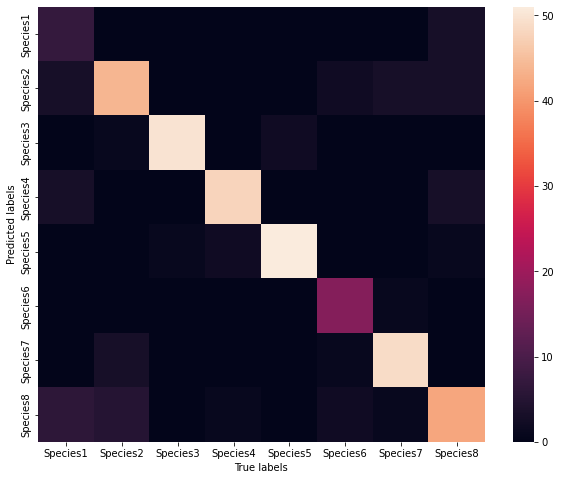
\includegraphics[width=\columnwidth]{VGG19_best}}
\caption{Confusion Matrix of best configuration with VGG19.}
\label{bayespic}
\end{center}
\end{figure}
\subsubsection{Considerations}
One of the most particular observation that we can made after experimenting the first attempts of freezing, is that freezing the net
until the pooling and not between convolutions leads to a better accuracy.

\subsection{Xception}

\subsection{Other Models}
\subsubsection{Resnet}
--NICOLA--
\subsubsection{GoogleNet}
\subsection{EfficientNet}
--NICOLA--



\section{Ensemble}
--NICOLA--
Approccio
provato a mischiare modelli
          c'era bias perché avevano seed diversi
\subsubsection{Results}



\section{If we had more time..}
con più tempo cosa avremmo provato




\section{Our Submissions}
\begin{table}[ht]
\centering
\begin{adjustbox}{width=240}
\small
\begin{tabular}{|c|l|l|l|l|l}

\hline \bf Model & \bf Details & \bf Result \\ \hline
VGG16 & 8 Freezed Layers & 0.8325 \\
VGG19 & 10 Freezed Layers & 0.8230 \\
\hline
\end{tabular}
\end{adjustbox}
\caption{Results with Transfer Learning and Number of freezed layers for VGG19.}
\end{table}
%{\bf Footnotes}: Note di sotto.}.
\section{Conclusions}
Considerazioni finali e best model fattoo
\bibliographystyle{sdss2020} % Please do not change the bibliography style
\bibliography{SampleReferencesForExtendedAbstract}

\end{document}
